\documentclass[aspectratio=169,10pt]{beamer}

\usetheme{Madrid}
\usecolortheme{seahorse}
% UTF-8 is default in modern LaTeX
\usepackage{amsmath,amssymb,amsfonts}
\usepackage{listings}
\usepackage{xcolor}
\usepackage{graphicx}
\usepackage{hyperref}

% Set graphics path
\graphicspath{{figures/}}

% Listing style for code
\lstset{
    basicstyle=\ttfamily\scriptsize,
    numbers=left,
    frame=single,
    breaklines=true,
    commentstyle=\color{green!50!black}\itshape,
    keywordstyle=\color{blue}\bfseries,
    stringstyle=\color{red},
    backgroundcolor=\color{gray!10},
    numberstyle=\tiny\color{gray},
}

% Footer with frame number
\setbeamertemplate{footline}[frame number]

% Document info
\title{Ishikawa Iteration and Common Fixed Point Theorems}
\subtitle{Chapter 5: Fixed Point Theorems (Pages 405-428)}
\author{Pathak's Fixed Point Theory}
\date{2024}

\begin{document}

% ============================================================================
% TITLE SLIDE
% ============================================================================
\frame{\titlepage}

% ============================================================================
% TABLE OF CONTENTS
% ============================================================================
\begin{frame}
\frametitle{Course Overview}
\tableofcontents
\end{frame}

% ============================================================================
% SECTION 1: INTRODUCTION AND MOTIVATION
% ============================================================================
\section{Introduction: Fixed Point Iteration Methods}

\begin{frame}[allowframebreaks]
\frametitle{What are Fixed Point Iteration Methods?}

\textbf{Definition:} A fixed point iteration method is a sequence of approximations to solve equations of the form:
$$x = T(x)$$

where $T: X \to X$ is a mapping on some space $X$.

\vspace{0.3cm}

\textbf{Key Question:} How do we find solutions to operator equations?

\vspace{0.3cm}

\textbf{Answer:} Using iteration schemes:
\begin{itemize}
    \item \textbf{One-step (Picard):} $x_{n+1} = Tx_n$
    \vspace{0.2cm}
    \item \textbf{Two-step (Ishikawa/Mann):} Involve multiple stages per iteration
    \vspace{0.2cm}
    \item \textbf{Multi-step:} Generalize to families of mappings
\end{itemize}

\vspace{0.3cm}

\textbf{Why use two-step methods?}
\begin{itemize}
    \item More flexible convergence conditions
    \item Applicable to broader classes of mappings
    \item Better stability properties
    \item Can handle nonexpansive mappings
\end{itemize}

\end{frame}

% ============================================================================
% SECTION 2: COMMON FIXED POINT THEOREMS
% ============================================================================
\section{Common Fixed Point Theorems (Section 5.5)}

\begin{frame}
\frametitle{Common Fixed Points: Definitions}

\textbf{Definition 5.66} (George et al.): Let $(X, d)$ be a metric space, $k$ a positive integer,
$T: X^k \to X$ and $f: X \to X$ be mappings.

\vspace{0.3cm}

\textbf{(a) Coincidence Point:}
$$x \in X \text{ is a coincidence point of } f \text{ and } T \iff f(x) = T(x, x, \ldots, x)$$

\vspace{0.3cm}

\textbf{(b) Common Fixed Point:}
$$x \text{ is a common fixed point} \iff x = f(x) = T(x, x, \ldots, x)$$

\vspace{0.3cm}

\textbf{(c) Commuting Mappings:}
$$f(T(x,x,\ldots,x)) = T(f(x), f(x), \ldots, f(x)) \quad \forall x \in X$$

\vspace{0.3cm}

\textbf{(d) Weakly Compatible:}
Mappings commute at their coincidence points.

\end{frame}

\begin{frame}
\frametitle{Theorem 5.118: Ćirić-Presić Type Theorem in b-Metric Spaces}

\textbf{Theorem 5.118:} Let $(X, d)$ be a b-metric space with $s \geq 1$.
For any positive integer $k$, let $f: X^k \to X$ and $g: X \to X$ satisfy:

\vspace{0.15cm}

\textbf{Conditions:}
\begin{itemize}
    \item[\textbf{(i)}] $f(X^k) \subseteq g(X)$

    \item[\textbf{(ii)}] $d(f(x_1, \ldots, x_k), f(x_2, \ldots, x_{k+1})) \leq \lambda \phi(d(gx_1, gx_2), \ldots, d(gx_k, gx_{k+1}))$
    \quad where $\lambda \in (0, 1/s^k)$

    \item[\textbf{(iii)}] $d(f(u,\ldots,u), f(v,\ldots,v)) < d(gu, gv)$ for all $u, v \in X$

    \item[\textbf{(iv)}] $g(X)$ is complete
\end{itemize}

\vspace{0.2cm}

\textbf{Conclusion:}
\begin{itemize}
    \item $f$ and $g$ have a unique common fixed point
    \item The sequence $\{y_n\}$ defined by $y_n = g(x_n) = f(x_n, x_{n+1}, \ldots, x_{n+k-1})$ converges to the common fixed point
\end{itemize}

\end{frame}

\begin{frame}
\frametitle{Common Fixed Points of Families of Mappings}

\textbf{Definition 5.67:} A mapping $F: K \to K$ on a convex subset of a normed linear space is:
$$\textbf{Affine} \iff F(\alpha x + (1-\alpha)y) = \alpha F(x) + (1-\alpha)F(y), \quad \alpha \in (0,1)$$

\vspace{0.3cm}

\textbf{Theorem 5.120 (Markov-Kakutani):} Let $K$ be a compact convex subset of a normed linear space $X$.
If $\mathcal{F}$ is a commuting family of continuous affine mappings of $K$ into itself, then there exists
$u \in K$ such that $Fu = u$ for all $F \in \mathcal{F}$.

\vspace{0.3cm}

\textbf{Applications:}
\begin{itemize}
    \item Solving systems of equations
    \item Equilibrium problems
    \item Game theory
\end{itemize}

\end{frame}

\begin{frame}
\frametitle{Theorem 5.123: de Marr's Theorem (Nonexpansive Mappings)}

\textbf{Theorem 5.123 (de Marr, 1963):} Let $K$ be a compact convex subset of a Banach space $X$,
and let $\mathcal{F}$ be a family of commuting nonexpansive mappings of $K$ into itself.
Then there is a common fixed point for the family.

\vspace{0.3cm}

\textbf{Definition:} A mapping $T: K \to K$ is \textbf{nonexpansive} if:
$$\|Tx - Ty\| \leq \|x - y\| \quad \forall x, y \in K$$

\vspace{0.3cm}

\textbf{Key Properties of Nonexpansive Mappings:}
\begin{itemize}
    \item More general than contractions
    \item No Lipschitz constant less than 1 required
    \item May not have unique fixed points
    \item Still have nice convergence properties under iteration
\end{itemize}

\vspace{0.3cm}

\textbf{Related Results:}
\begin{itemize}
    \item \textbf{Theorem 5.126 (Browder):} Nonexpansive families have common fixed points in uniformly convex Banach spaces
    \item \textbf{Theorem 5.124-5.125:} Variations for weakly compact and bounded convex sets
\end{itemize}

\end{frame}

% ============================================================================
% SECTION 3: ITERATION SCHEMES FOR COMMON FIXED POINTS
% ============================================================================
\section{Iteration Schemes for Common Fixed Points}

\begin{frame}
\frametitle{Iteration Schemes: General Framework}

\textbf{Problem:} Find a common fixed point of a family $\{F_i\}_{i=1}^k$ of nonexpansive mappings.

\vspace{0.3cm}

\textbf{Approach:} Define an iteration scheme using weighted averages:

\vspace{0.15cm}

For $0 < \alpha < 1$, define operators:
\begin{align*}
U_0 &= I \quad \text{(identity mapping)} \\
U_r &= (1-\alpha)I + \alpha F_r U_{r-1}, \quad r = 1, 2, \ldots, k
\end{align*}

\vspace{0.3cm}

The iteration scheme generates a sequence by repeatedly applying $U_k$:
$$\{U_k^n(x)\}_{n=1}^{\infty}$$

\vspace{0.3cm}

\textbf{Interpretation:}
\begin{itemize}
    \item Each $U_r$ is a convex combination of identity and the mapped previous operator
    \item The combined operator $U_k$ applies all $k$ mappings in sequence
    \item Linearly weighted by parameter $\alpha$
\end{itemize}

\end{frame}

\begin{frame}
\frametitle{Theorem 5.130: Strong Convergence}

\textbf{Theorem 5.130:} Let $K$ be a compact convex subset of a strictly convex Banach space $X$,
and $\{F_i\}_{i=1}^k$ a finite family of nonexpansive self-mappings of $K$ with nonempty common fixed point set.

\vspace{0.2cm}

Then for any $x \in K$, the sequence $\{U_k^n(x)\}_{n=1}^{\infty}$ \textbf{converges strongly}
to a common fixed point of $\{F_i\}_{i=1}^k$.

\vspace{0.3cm}

\textbf{Proof Strategy:}
\begin{enumerate}
    \item Show $U_k$ is nonexpansive: $\|U_k(x) - U_k(y)\| \leq \|x - y\|$
    \item Use Edelstein's theorem for contraction properties
    \item Exploit strict convexity for strong convergence
    \item Bounded sequences in finite dimensions converge
\end{enumerate}

\vspace{0.3cm}

\textbf{Key Requirement:} Strict convexity of the space (e.g., Hilbert spaces, $L^p$ spaces with $p > 1$)

\end{frame}

\begin{frame}
\frametitle{Theorem 5.131: Weak Convergence}

\textbf{Theorem 5.131:} If $X$ is a uniformly convex Banach space satisfying Opial's condition
(e.g., Hilbert spaces), let $K$ be closed and convex, and $\{F_i\}_{i=1}^k$ a family of nonexpansive
self-mappings of $K$ with nonempty common fixed point set.

\vspace{0.2cm}

Then for any $x \in K$, the sequence $\{U_k^n(x)\}_{n=1}^{\infty}$ \textbf{converges weakly}
to a common fixed point.

\vspace{0.3cm}

\textbf{Opial's Condition:} For any sequence $\{x_n\}$ and $x \in X$:
$$\limsup_{n \to \infty} \|x_n - x\| < \limsup_{n \to \infty} \|x_n - y\|, \quad \text{whenever } x_n \rightharpoonup x \text{ and } x \neq y$$

\vspace{0.3cm}

\textbf{Examples of spaces satisfying Opial's condition:}
\begin{itemize}
    \item All Hilbert spaces
    \item $\ell^p$ spaces for $1 \leq p < \infty$
    \item But NOT $L^p$ spaces for $p \neq 2$
\end{itemize}

\end{frame}

\begin{frame}[fragile]
\frametitle{Theorem 5.132: Parameter-Controlled Convergence}

\textbf{Theorem 5.132:} Let $K$ be closed and convex in a uniformly convex Banach space $X$ with Fréchet differentiable norm.
Let $\{F_i\}_{i=1}^k$ be nonexpansive self-mappings with nonempty fixed point set, and $\{c_n\}$ a sequence with:

\vspace{0.2cm}

\textbf{Conditions on sequence $\{c_n\}$:}
\begin{itemize}
    \item[\textbf{(i)}] $0 \leq c_n \leq 1$
    \item[\textbf{(ii)}] $\sum_{n=1}^{\infty} c_n(1 - c_n) = \infty$
\end{itemize}

\vspace{0.2cm}

Define the iteration:
$$x_{n+1} = (1-c_n)x_n + c_n F_k U_{k-1} x_n, \quad n \geq 1$$

\vspace{0.2cm}

Then $\{x_n\}$ \textbf{converges weakly} to a common fixed point of $\{F_i\}_{i=1}^k$.

\vspace{0.3cm}

\textbf{Interpretation:}
\begin{itemize}
    \item Parameter $c_n$ controls step size at each iteration
    \item Condition (ii) ensures sufficient exploration (not too greedy)
    \item Relates to gradient descent and optimization methods
\end{itemize}

\vspace{0.2cm}

\textbf{Example parameters:} $c_n = 1/(n+1)$, $c_n = 1/\sqrt{n}$

\end{frame}

\begin{frame}[allowframebreaks]
\frametitle{Application: System of Operator Equations}

\textbf{Problem:} Solve a system of operator equations:
$$x - T_i x = f_i, \quad i = 1, 2, \ldots, k$$

where $T_i$ are nonexpansive and $f_i$ are given elements.

\vspace{0.3cm}

\textbf{Solution Approach:} Define the family of mappings:
$$F_i(x) = f_i + T_i(x), \quad i = 1, 2, \ldots, k$$

\vspace{0.3cm}

\textbf{Key Observation:}
\begin{itemize}
    \item $x$ is a solution to the system $\iff$ $x$ is a common fixed point of $\{F_i\}_{i=1}^k$
    \item Each $F_i$ is nonexpansive (since $T_i$ is nonexpansive)
    \item Apply Theorems 5.130, 5.131, or 5.132 to find the solution iteratively
\end{itemize}

\vspace{0.3cm}

\textbf{Algorithm (Theorem 5.132):}

\small
\texttt{
\begin{tabular}{l}
x = x\_initial \\
\textbf{for} n = 1, 2, $\ldots$: \\
\quad \# Compute weighted averages \\
\quad U = I \\
\quad \textbf{for} r = 1, $\ldots$, k: \\
\quad \quad U = $(1 - \alpha)$I $+$ $\alpha F_r U$ \\
\quad \# Apply parameter-controlled step \\
\quad $c_n = 1/(n+1)$ \\
\quad x = $(1-c_n)$x $+ c_n F_k U$ x \\
\quad \textbf{if} converged(x): \textbf{break}
\end{tabular}
}
\normalsize

\end{frame}

% ============================================================================
% SECTION 4: SEQUENCES OF CONTRACTIONS AND GENERALIZATIONS
% ============================================================================
\section{Sequences of Contractions and Generalizations (Section 5.6)}

\begin{frame}
\frametitle{Fixed Points of Contraction Sequences}

\textbf{Question:} If $\{F_n\}$ is a sequence of contractions converging to $F$, do their fixed points converge to a fixed point of $F$?

\vspace{0.3cm}

\textbf{Answer:} YES, under appropriate conditions!

\vspace{0.3cm}

\textbf{Theorem 5.133 (Bonsall, 1962):} Let $(X, d)$ be a complete metric space, and let $T$ and $T_n$
($n = 1, 2, \ldots$) be contraction mappings with the same Lipschitz constant $k < 1$ and fixed points $u$ and $u_n$ respectively.

\vspace{0.2cm}

If $\lim_{n \to \infty} T_n x = T x$ for every $x \in X$, then $\lim_{n \to \infty} u_n = u$.

\vspace{0.3cm}

\textbf{Proof Sketch:}
\begin{enumerate}
    \item Use Banach contraction principle: $d(u_n, T_n^m x_0) \leq \frac{k^m}{1-k} d(T_n x_0, x_0)$
    \item Set $m = 0$ and $x_0 = u$: $d(u_n, u) \leq \frac{1}{1-k} d(T_n u, u)$
    \item Take limit as $n \to \infty$: $\lim_{n \to \infty} d(u_n, u) = 0$
\end{enumerate}

\vspace{0.3cm}

\textbf{Applications:}
\begin{itemize}
    \item Perturbation analysis
    \item Stability of numerical schemes
    \item Continuity of solutions under parameter changes
\end{itemize}

\end{frame}

\begin{frame}
\frametitle{Multivalued Mappings and Hausdorff Metric}

\textbf{Definition:} For nonempty closed subsets of $X$, the Hausdorff metric is:
$$H(A, B) = \max\{\sup_{x \in A} d(x, B), \sup_{y \in B} d(y, A)\}$$

\vspace{0.3cm}

\textbf{Theorem 5.127 (Bose-Mukerjee):} Let $(X, d)$ be a complete bounded metric space,
and $F_i: X \to \text{CL}(X)$ (multivalued mappings to closed sets) satisfy:

\vspace{0.15cm}

$$H(F_1(x), F_2(y)) \leq a_1 d(x, F_1(x)) + a_2 d(y, F_2(y)) + a_3 d(y, F_1(x)) + a_4 d(x, F_2(y)) + a_5 d(x, y)$$

where $\sum_{i=1}^5 a_i < 1$ and $a_1 = a_2$ or $a_3 = a_4$.

\vspace{0.2cm}

Then $F_1$ and $F_2$ have a common fixed point.

\vspace{0.3cm}

\textbf{Key Features:}
\begin{itemize}
    \item Generalizes Kannan-Reich condition to multivalued mappings
    \item Allows non-contractive mappings
    \item Oscillating (alternating) indices $i, j$ in sequence
    \item Distance to set (not just point) appears in condition
\end{itemize}

\end{frame}

% ============================================================================
% SECTION 5: ISHIKAWA ITERATION DETAILS
% ============================================================================
\section{Ishikawa Iteration and Two-Step Methods}

\begin{frame}
\frametitle{Ishikawa Iteration: Definition}

\textbf{Definition:} The Ishikawa iteration for a mapping $T: K \to K$ on a convex subset $K$
of a Banach space is defined as follows:

\vspace{0.3cm}

For a given $x_0 \in K$ and sequences $\{\alpha_n\}$, $\{\beta_n\}$ in $(0,1)$:

\vspace{0.15cm}

\textbf{Two-step scheme:}
\begin{align}
y_n &= (1 - \alpha_n) x_n + \alpha_n T x_n \label{eq:ishikawa1} \\
x_{n+1} &= (1 - \beta_n) x_n + \beta_n T y_n \label{eq:ishikawa2}
\end{align}

\vspace{0.3cm}

\textbf{Notation:}
\begin{itemize}
    \item $\alpha_n, \beta_n$: step-size parameters (usually in $(0, 1)$)
    \item $y_n$: intermediate iterate (first step)
    \item $x_{n+1}$: next iterate (second step)
    \item $T$: the nonexpansive mapping
\end{itemize}

\vspace{0.3cm}

\textbf{Special Cases:}
\begin{itemize}
    \item $\alpha_n = 0$: Reduces to Mann iteration (with parameter $\beta_n$)
    \item $\alpha_n = \beta_n = 1$: Reduces to Picard iteration $x_{n+1} = T(x_n)$
\end{itemize}

\end{frame}

\begin{frame}
\frametitle{Convergence of Ishikawa Iteration}

\textbf{Theorem (Ishikawa, 1974):} Let $K$ be a closed, bounded, convex subset of a uniformly convex
Banach space $X$. Let $T: K \to K$ be a nonexpansive mapping. Then for sequences $\{\alpha_n\}$ and $\{\beta_n\}$
with:

\vspace{0.15cm}

\textbf{Conditions:}
\begin{enumerate}
    \item $0 < a \leq \alpha_n, \beta_n \leq b < 1$ for all $n$
    \item $\sum_{n=1}^{\infty} \alpha_n = \infty$ and $\sum_{n=1}^{\infty} \beta_n = \infty$
\end{enumerate}

The Ishikawa sequence $\{x_n\}$ \textbf{converges weakly} to a fixed point of $T$.

\vspace{0.3cm}

\textbf{Key Advantages:}
\begin{itemize}
    \item Works for nonexpansive mappings (not just contractions)
    \item More flexibility in choosing parameters
    \item Applicable to fixed point problems in infinite-dimensional spaces
    \item Better numerical stability in some cases
\end{itemize}

\vspace{0.3cm}

\textbf{Comparison with Picard:}
\begin{itemize}
    \item Picard: $x_{n+1} = Tx_n$ (simpler, faster for contractions)
    \item Ishikawa: Two-step (more robust for nonexpansive maps)
\end{itemize}

\end{frame}

\begin{frame}
\frametitle{Mann Iteration (Special Case)}

\textbf{Definition:} The Mann iteration is obtained from Ishikawa with $\alpha_n = 0$:

\vspace{0.3cm}

$$x_{n+1} = (1 - \beta_n) x_n + \beta_n T x_n = x_n + \beta_n (T x_n - x_n)$$

\vspace{0.3cm}

\textbf{Interpretation:}
\begin{itemize}
    \item No intermediate step, direct convex combination
    \item $\beta_n$ controls how much we move toward $T x_n$
    \item $\beta_n$ small $\Rightarrow$ slow convergence but stable
    \item $\beta_n$ large $\Rightarrow$ faster but potentially unstable
\end{itemize}

\vspace{0.3cm}

\textbf{Convergence (Mann):} Under similar conditions, Mann iteration also converges weakly to a fixed point.

\vspace{0.3cm}

\textbf{Practical Choices:}
\begin{itemize}
    \item Constant: $\beta_n = \beta \in (0,1)$ for all $n$ (simple, often $\beta = 0.5$)
    \item Decreasing: $\beta_n = 1/n$ or $\beta_n = 1/\sqrt{n}$ (theoretical guarantee)
    \item Adaptive: Choose $\beta_n$ based on convergence progress
\end{itemize}

\end{frame}

% ============================================================================
% SECTION 6: VISUALIZATION AND EXAMPLES
% ============================================================================
\section{Visualization and Examples}

\begin{frame}
\frametitle{Visual Comparison: Iteration Schemes}

\centering
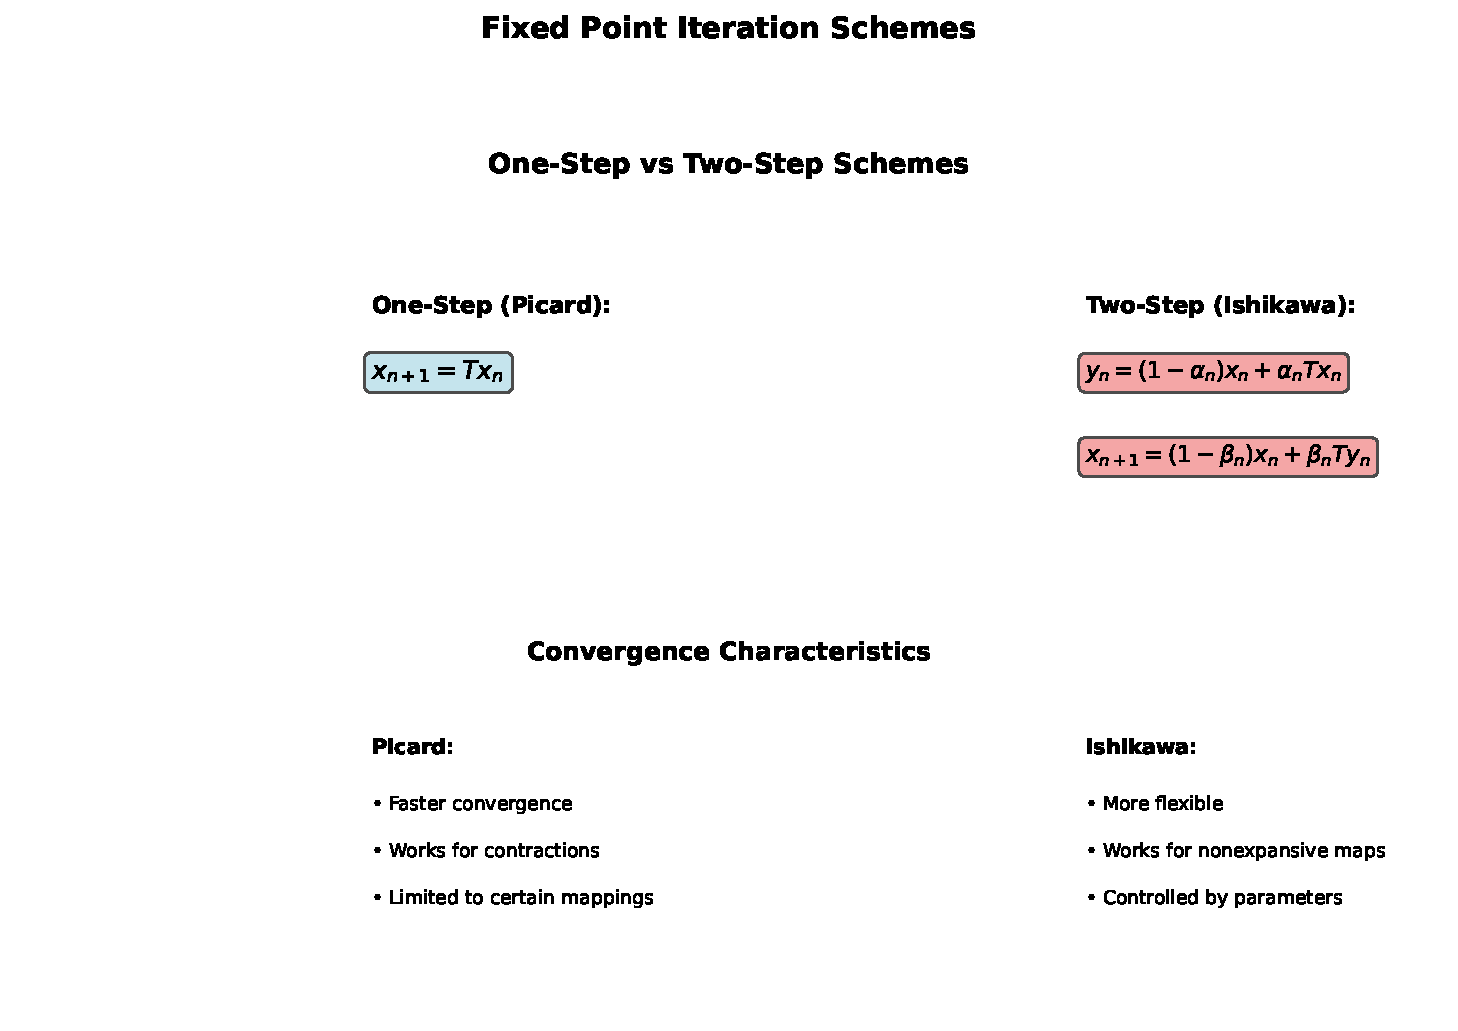
\includegraphics[width=0.95\textwidth]{01_iteration_schemes}

\end{frame}

\begin{frame}
\frametitle{Convergence Behavior: Numerical Example}

\centering
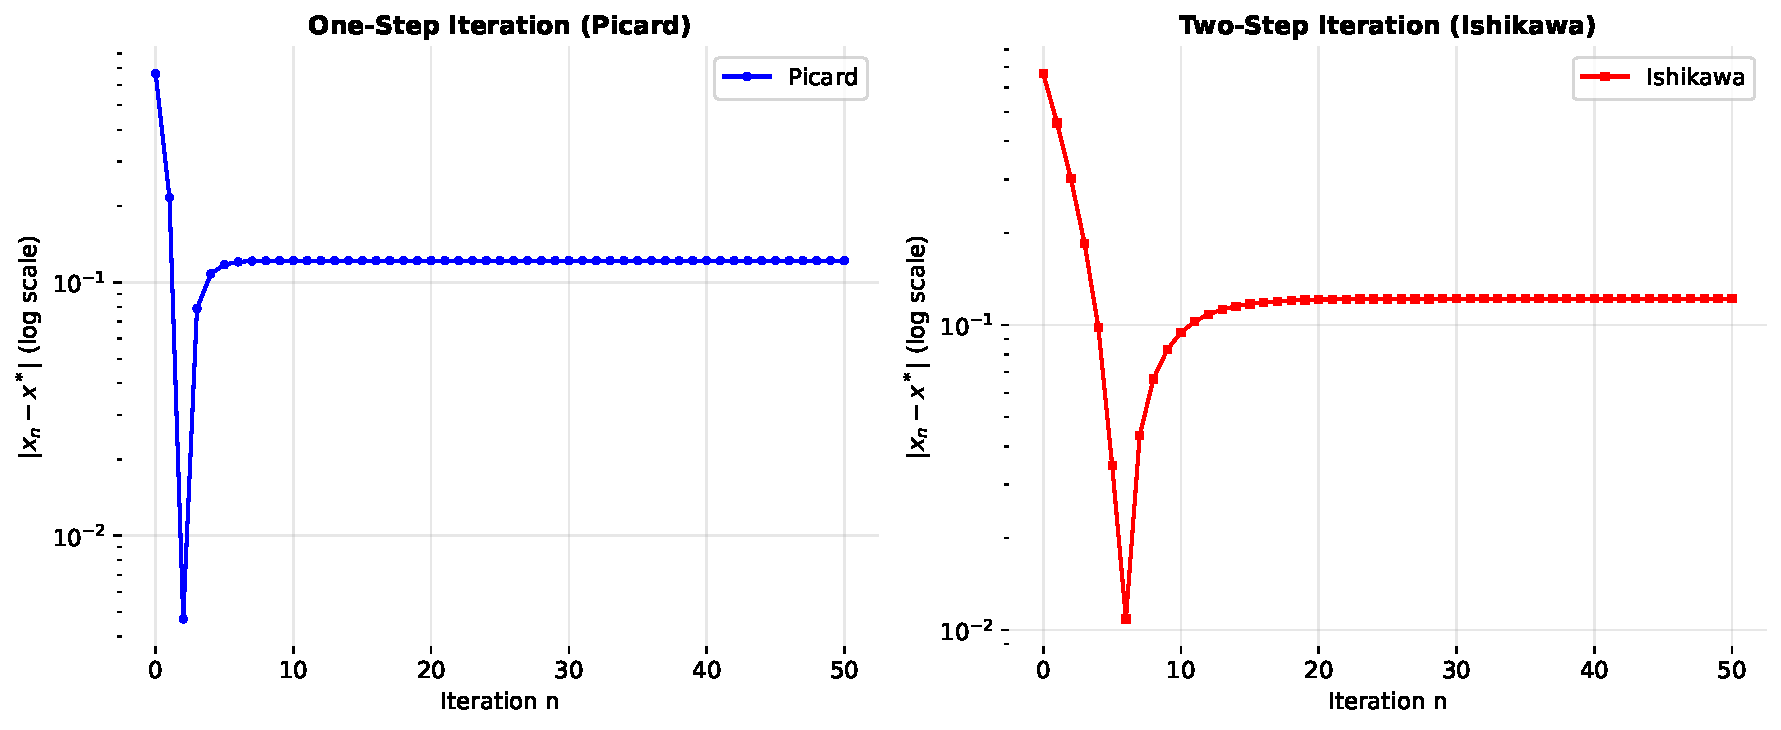
\includegraphics[width=0.95\textwidth]{02_convergence_comparison}

\end{frame}

\begin{frame}
\frametitle{Nonexpansive Mapping Property}

\centering
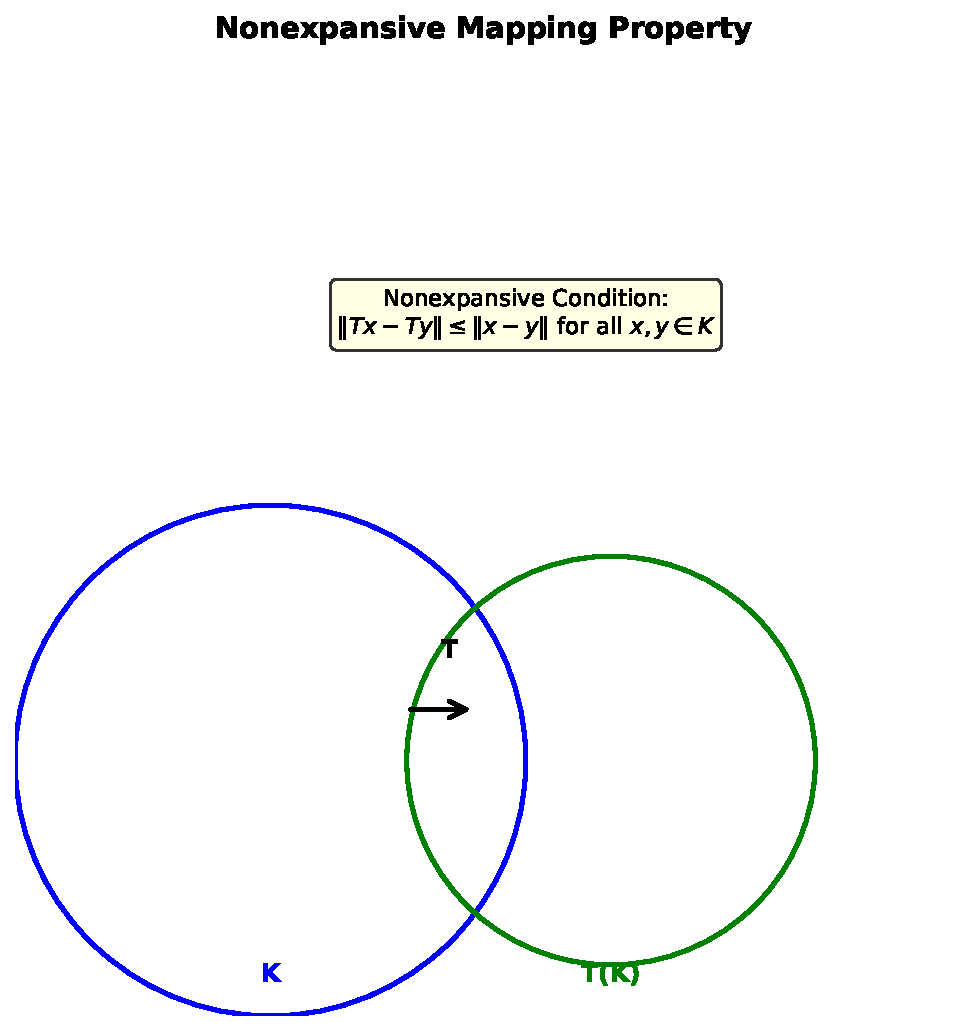
\includegraphics[width=0.9\textwidth]{03_nonexpansive_mapping}

\vspace{0.3cm}

The nonexpansive property $\|Tx - Ty\| \leq \|x - y\|$ is weaker than contraction but still allows fixed points.

\end{frame}

\begin{frame}
\frametitle{Fixed Point Theorem Structure}

\centering
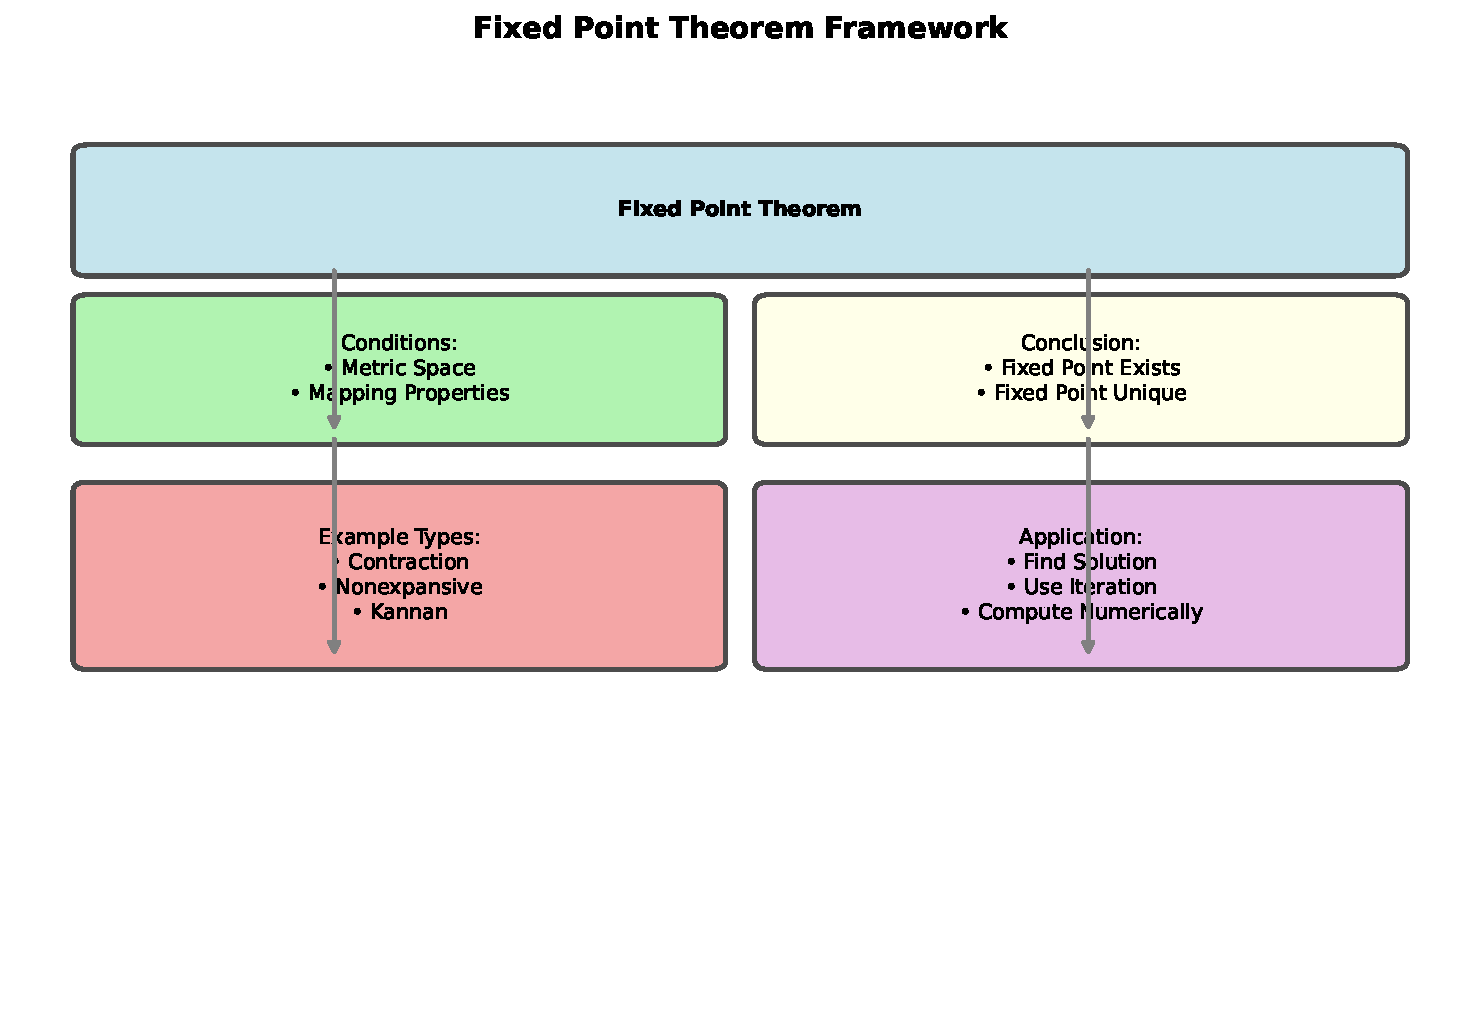
\includegraphics[width=0.95\textwidth]{04_theorem_structure}

\end{frame}

\begin{frame}
\frametitle{Parameter Sensitivity in Ishikawa Iteration}

\centering
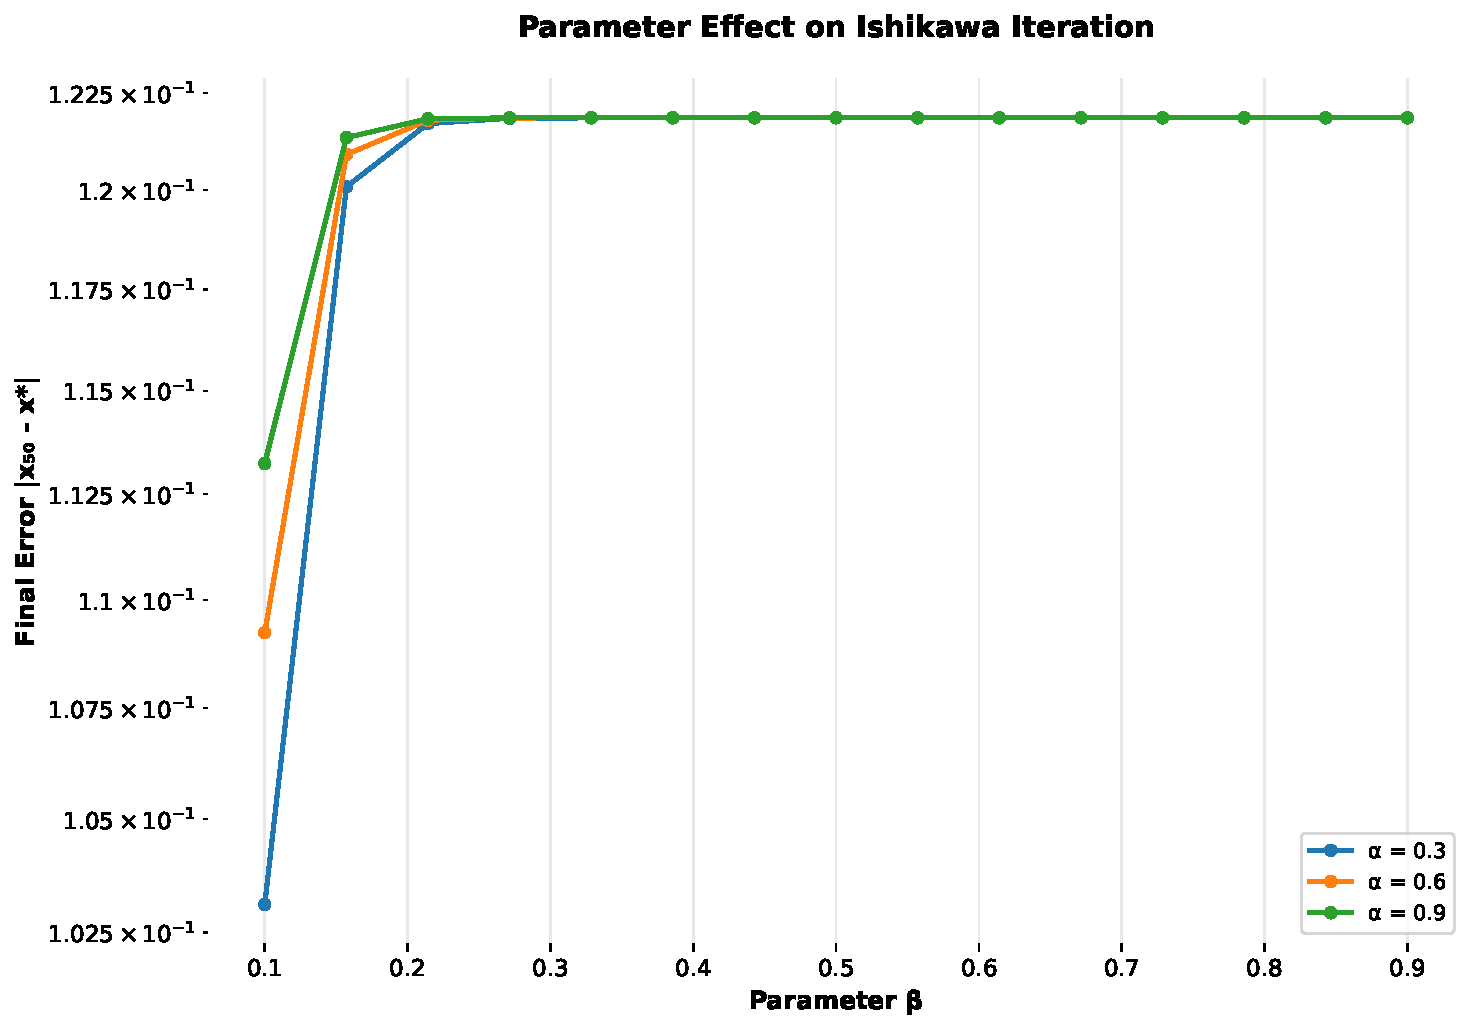
\includegraphics[width=0.95\textwidth]{05_parameter_sensitivity}

\vspace{0.3cm}

Final error after 50 iterations depends on both $\alpha$ and $\beta$ parameters.
Optimal choice requires problem-specific tuning.

\end{frame}

\begin{frame}
\frametitle{b-Metric Space Illustration}

\centering
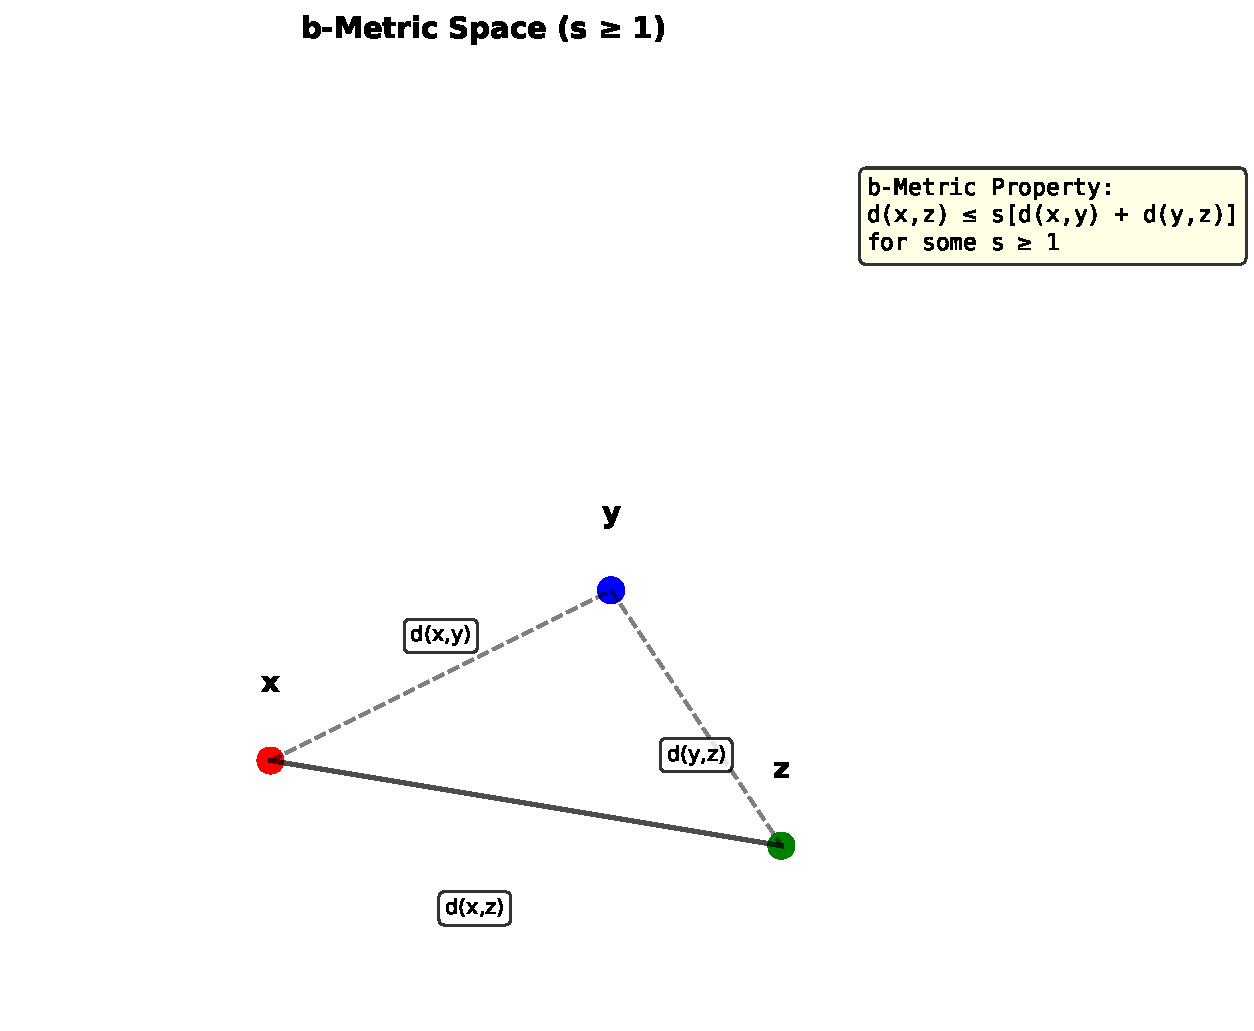
\includegraphics[width=0.9\textwidth]{06_bmetric_space}

\end{frame}

\begin{frame}
\frametitle{Convergence Rates Comparison}

\centering
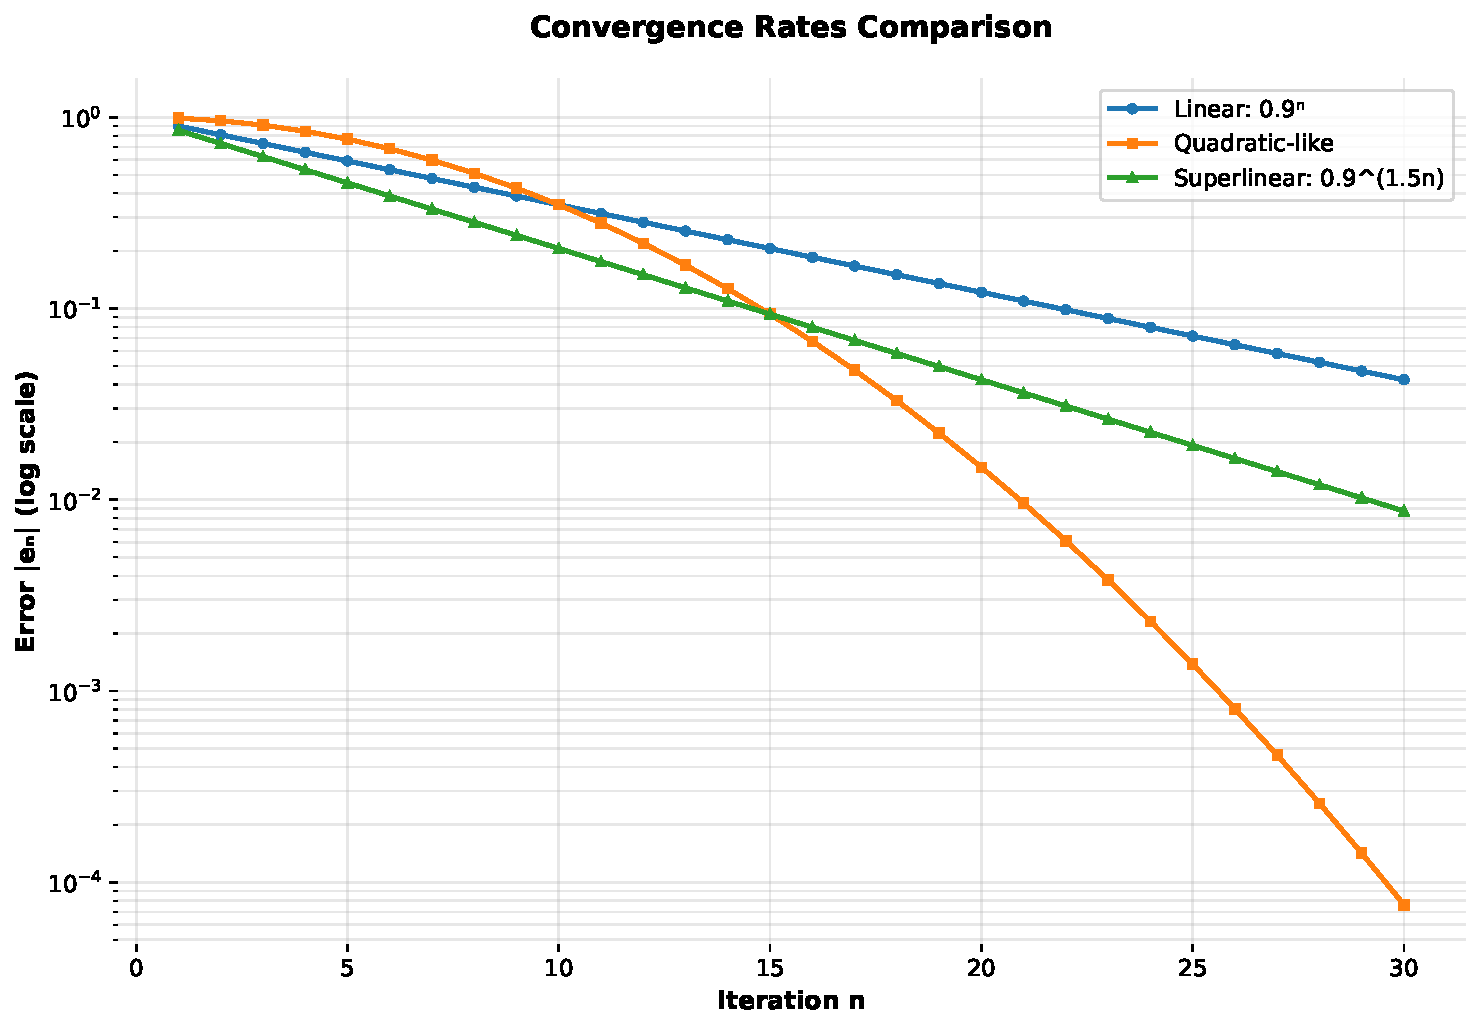
\includegraphics[width=0.95\textwidth]{07_convergence_rates}

\vspace{0.3cm}

Different iteration methods exhibit different convergence rates: linear, superlinear, or quadratic.

\end{frame}

% ============================================================================
% SECTION 7: NUMERICAL IMPLEMENTATION
% ============================================================================
\section{Numerical Implementation}

\begin{frame}[fragile]
\frametitle{Python Implementation: Ishikawa Iteration}

\small
{\ttfamily
\begin{tabular}{l}
import numpy as np \\
\\
def ishikawa(T, x0, alpha, beta, maxit=100): \\
\quad x = float(x0) \\
\quad for n in range(maxit): \\
\quad \quad y = (1-alpha)*x + alpha*T(x) \\
\quad \quad x\_new = (1-beta)*x + beta*T(y) \\
\quad \quad if abs(x\_new - x) $<$ 1e-8: \\
\quad \quad \quad return x\_new, n \\
\quad \quad x = x\_new \\
\quad return x, maxit \\
\\
x\_star, iters = ishikawa(T, 0.1, 0.4, 0.6) \\
\end{tabular}
}

\end{frame}

\begin{frame}
\frametitle{Common Fixed Point Problem (Theorem 5.132)}

\textbf{Solve system:} $x - T_i(x) = f_i$ for $i=1,\ldots,k$

\vspace{0.2cm}

\textbf{Algorithm:}
\begin{enumerate}
    \item Define $F_i(x) = f_i + T_i(x)$ (nonexpansive)
    \item Compute weighted operators: $U_r = (1-\alpha)I + \alpha F_r U_{r-1}$
    \item Apply parameter-controlled iteration:
    \vspace{0.1cm}
    $$x_{n+1} = (1-c_n)x_n + c_n F_k U_{k-1}(x_n)$$
    where $c_n \to 0$ and $\sum_n c_n(1-c_n) = \infty$
\end{enumerate}

\vspace{0.3cm}

\textbf{Pseudocode:}

\small
\texttt{
\begin{tabular}{l}
for $n = 1, 2, \ldots$: \\
\quad Compute $U_r = (1-\alpha)I + \alpha F_r U_{r-1}$ for $r = 1,\ldots,k$ \\
\quad Set $c_n = 1/(n+1)$ \\
\quad $x_{n+1} \leftarrow (1-c_n)x_n + c_n F_k U_{k-1}(x_n)$ \\
\quad if $|x_{n+1} - x_n| < \epsilon$: break \\
\text{return } $x_{n+1}$
\end{tabular}
}
\normalsize

\vspace{0.2cm}

\textbf{Convergence:} Weakly to a common fixed point of all $F_i$.

\end{frame}

\end{frame}

% ============================================================================
% SECTION 8: APPLICATIONS
% ============================================================================
\section{Applications and Extensions}

\begin{frame}
\frametitle{Key Applications}

\textbf{1. Solving Operator Equations:}
\begin{itemize}
    \item $x - Tx = f$ (Lax-Milgram theory)
    \item Nonlinear elliptic PDEs
    \item Integral equations of Fredholm type
\end{itemize}

\vspace{0.3cm}

\textbf{2. Variational Inequalities:}
\begin{itemize}
    \item $\langle Ax - b, x - y \rangle \geq 0$ for all $y$ in a convex set
    \item Can be reformulated as fixed point problems
    \item Applications in optimization and game theory
\end{itemize}

\vspace{0.3cm}

\textbf{3. Machine Learning:}
\begin{itemize}
    \item Federated learning with local and global updates (Ishikawa-type)
    \item Consensus algorithms for distributed optimization
    \item Deep learning: momentum-based optimization (related to two-step methods)
\end{itemize}

\vspace{0.3cm}

\textbf{4. Numerical Linear Algebra:}
\begin{itemize}
    \item Iterative methods for solving $Ax = b$
    \item Eigenvalue problems
    \item Matrix fixed points
\end{itemize}

\vspace{0.3cm}

\textbf{5. Control Theory:}
\begin{itemize}
    \item Equilibrium problems in dynamical systems
    \item Stability analysis of discrete-time systems
\end{itemize}

\end{frame}

\begin{frame}
\frametitle{Practical Considerations}

\textbf{When to use which method?}

\vspace{0.2cm}

\textbf{Picard iteration ($x_{n+1} = Tx_n$):}
\begin{itemize}
    \item [+] $T$ is a contraction mapping ($k < 1$)
    \item [+] Need fast convergence
    \item [-] Limited to certain mapping classes
    \item [-] May diverge for nonexpansive mappings
\end{itemize}

\vspace{0.2cm}

\textbf{Mann iteration:}
\begin{itemize}
    \item [+] $T$ is nonexpansive
    \item [+] Want convergence guarantees
    \item [~] Slower than Picard but more robust
    \item [+] Easier to implement than Ishikawa
\end{itemize}

\vspace{0.2cm}

\textbf{Ishikawa iteration:}
\begin{itemize}
    \item [+] $T$ is nonexpansive or quasi-nonexpansive
    \item [+] Need more control over iteration
    \item [+] Better stability properties
    \item [~] Two steps per iteration (slower per step)
    \item [+] More parameters to tune
\end{itemize}

\vspace{0.2cm}

\textbf{Parameter Selection Guidelines:}
\begin{itemize}
    \item Start with $\alpha_n = \beta_n = 0.5$ (middle values)
    \item Use decreasing sequences: $\alpha_n, \beta_n = 1/(n+1)$ or $1/\sqrt{n}$
    \item Problem-dependent tuning often needed
    \item Adaptive schemes: adjust parameters based on convergence rate
\end{itemize}

\end{frame}

% ============================================================================
% SECTION 9: SUMMARY AND CONCLUSIONS
% ============================================================================
\section{Summary and Conclusions}

\begin{frame}
\frametitle{Main Results Summary}

\textbf{Fixed Point Theorems (Section 5.5):}
\begin{itemize}
    \item \textbf{Theorem 5.118:} Ćirić-Presić in b-metric spaces
    \item \textbf{Theorem 5.120:} Markov-Kakutani (affine mappings)
    \item \textbf{Theorem 5.123:} de Marr (nonexpansive families)
    \item \textbf{Theorems 5.126, 5.124-5.125:} Browder, Belluce-Kirk generalizations
\end{itemize}

\vspace{0.3cm}

\textbf{Iteration Schemes (Section 5.5):}
\begin{itemize}
    \item \textbf{Theorem 5.130:} Strong convergence (compact strictly convex space)
    \item \textbf{Theorem 5.131:} Weak convergence (uniformly convex with Opial condition)
    \item \textbf{Theorem 5.132:} Parameter-controlled convergence
    \item Application to solving systems of operator equations
\end{itemize}

\vspace{0.3cm}

\textbf{Contraction Sequences (Section 5.6):}
\begin{itemize}
    \item \textbf{Theorem 5.133:} Continuity of fixed points under contraction sequences
    \item \textbf{Theorem 5.127:} Multivalued Kannan-Reich type mappings
\end{itemize}

\end{frame}

\begin{frame}
\frametitle{Key Conceptual Insights}

\textbf{1. Generalization Hierarchy:}
$$\text{Contraction} \subset \text{Nonexpansive} \subset \text{Quasi-nonexpansive} \subset \text{General mappings}$$

\vspace{0.3cm}

\textbf{2. Iteration Method Progression:}
$$\text{Picard} \subset \text{Mann} \subset \text{Ishikawa} \subset \text{General Multi-step}$$

\vspace{0.3cm}

\textbf{3. Convergence Trade-offs:}
\begin{itemize}
    \item Stronger mapping classes $\Rightarrow$ stronger convergence (strong vs. weak)
    \item More complex iteration $\Rightarrow$ wider applicability but slower per step
    \item Parameter tuning can balance convergence rate and stability
\end{itemize}

\vspace{0.3cm}

\textbf{4. Space Geometry Matters:}
\begin{itemize}
    \item \textbf{Strict convexity:} Enables strong convergence
    \item \textbf{Uniform convexity:} Stronger results, applies to more spaces
    \item \textbf{Opial condition:} Allows weak convergence analysis
\end{itemize}

\vspace{0.3cm}

\textbf{5. Common Fixed Points vs. Individual Fixed Points:}
\begin{itemize}
    \item Finding common fixed point of family $\{F_i\}$ often easier than sequential finding
    \item Weighted averaging (through $U_r$ operators) is key technique
\end{itemize}

\end{frame}

\begin{frame}
\frametitle{Research Directions and Open Problems}

\textbf{Extensions and Generalizations:}
\begin{itemize}
    \item Higher-order schemes (three-step, multi-step)
    \item Iteration for set-valued mappings
    \item Parallel and distributed iteration schemes
    \item Adaptive parameter selection strategies
\end{itemize}

\vspace{0.3cm}

\textbf{Theoretical Questions:}
\begin{itemize}
    \item Rate of convergence (linear vs. superlinear)
    \item Optimal parameter choices
    \item Convergence in exotic spaces (non-reflexive, non-locally convex, etc.)
\end{itemize}

\vspace{0.3cm}

\textbf{Computational Aspects:}
\begin{itemize}
    \item Efficient implementation on parallel/GPU hardware
    \item Error analysis and backward stability
    \item Preconditioning and acceleration techniques
\end{itemize}

\vspace{0.3cm}

\textbf{Applications:}
\begin{itemize}
    \item Machine learning: convergence analysis of distributed methods
    \item Image processing: iteration schemes for inverse problems
    \item Signal processing: frame expansions via fixed points
\end{itemize}

\end{frame}

\begin{frame}
\frametitle{Conclusion}

\textbf{Summary:}
\begin{itemize}
    \item Fixed point theorems provide existence and uniqueness results
    \item Iteration methods provide computational schemes to find fixed points
    \item Ishikawa iteration is a powerful two-step method applicable to nonexpansive mappings
    \item Parameter selection and space geometry play crucial roles
\end{itemize}

\vspace{0.4cm}

\textbf{Takeaway Message:}

\Large
\centering
\textbf{\textit{``Two-step iteration methods like Ishikawa provide a powerful balance between}}
\textbf{\textit{generality and computational feasibility.''}}

\vspace{0.4cm}

\normalsize
\raggedright

\textbf{Reading Recommendations:}
\begin{itemize}
    \item Pathak: Chapters 5.5-5.7 on fixed point theorems
    \item Ishikawa (1974): Original paper on two-step iterations
    \item Browder (1965+): Classic work on nonexpansive mappings in Banach spaces
    \item Recent reviews on machine learning applications
\end{itemize}

\end{frame}

\end{document}
